%%% This LaTeX source document can be used as the basis for your technical
%%% report. Intentionally stripped and simplified
%%% and commands should be adjusted for your particular paper - title, 
%%% author, citations, equations, etc.
% % Citations/references are in report.bib 

\documentclass[conference]{acmsiggraph}

\usepackage{graphicx}
\graphicspath{{./images/}}
\newcommand{\figuremacroW}[4]{
	\begin{figure}[h] %[htbp]
		\centering
		\includegraphics[width=#4\columnwidth]{#1}
		\caption[#2]{\textbf{#2} - #3}
		\label{fig:#1}
	\end{figure}
}

\newcommand{\figuremacroF}[4]{
	\begin{figure*}[h] % [htbp]
		\centering
		\includegraphics[width=#4\textwidth]{#1}
		\caption[#2]{\textbf{#2} - #3}
		\label{fig:#1}
	\end{figure*}
}


\usepackage{lipsum}

\usepackage{xcolor}
\definecolor{lbcolor}{rgb}{0.98,0.98,0.98}
\usepackage{listings}

\lstset{
	escapeinside={/*@}{@*/},
	language=C,
	basicstyle=\fontsize{8.5}{12}\selectfont,
	numbers=left,
	numbersep=2pt,    
	xleftmargin=2pt,
	%numberstyle=\tiny,
	frame=tb,
	%frame=single,
	columns=fullflexible,
	showstringspaces=false,
	tabsize=4,
	keepspaces=true,
	showtabs=false,
	showspaces=false,
	%showstringspaces=true
	backgroundcolor=\color{lbcolor},
	morekeywords={inline,public,class,private,protected,struct},
	captionpos=t,
	lineskip=-0.4em,
	aboveskip=10pt,
	%belowskip=50pt,
	extendedchars=true,
	breaklines=true,
	prebreak = \raisebox{0ex}[0ex][0ex]{\ensuremath{\hookleftarrow}},
	keywordstyle=\color[rgb]{0,0,1},
	commentstyle=\color[rgb]{0.133,0.545,0.133},
	stringstyle=\color[rgb]{0.627,0.126,0.941},
}


\TOGonlineid{45678}
\TOGvolume{0}
\TOGnumber{0}
\TOGarticleDOI{1111111.2222222}
\TOGprojectURL{}
\TOGvideoURL{}
\TOGdataURL{}
\TOGcodeURL{}

\title{An OpenGl Desert Scene}

\author{Sam Serrels\\\ 40082367@napier.ac.uk \\
Edinburgh Napier University\\
Computer Graphics (SET08116)}
\pdfauthor{Sam Serrels}

\keywords{OpenGL, GLSL, Graphics, SSBO, Reflections}

\begin{document}

\teaser{
   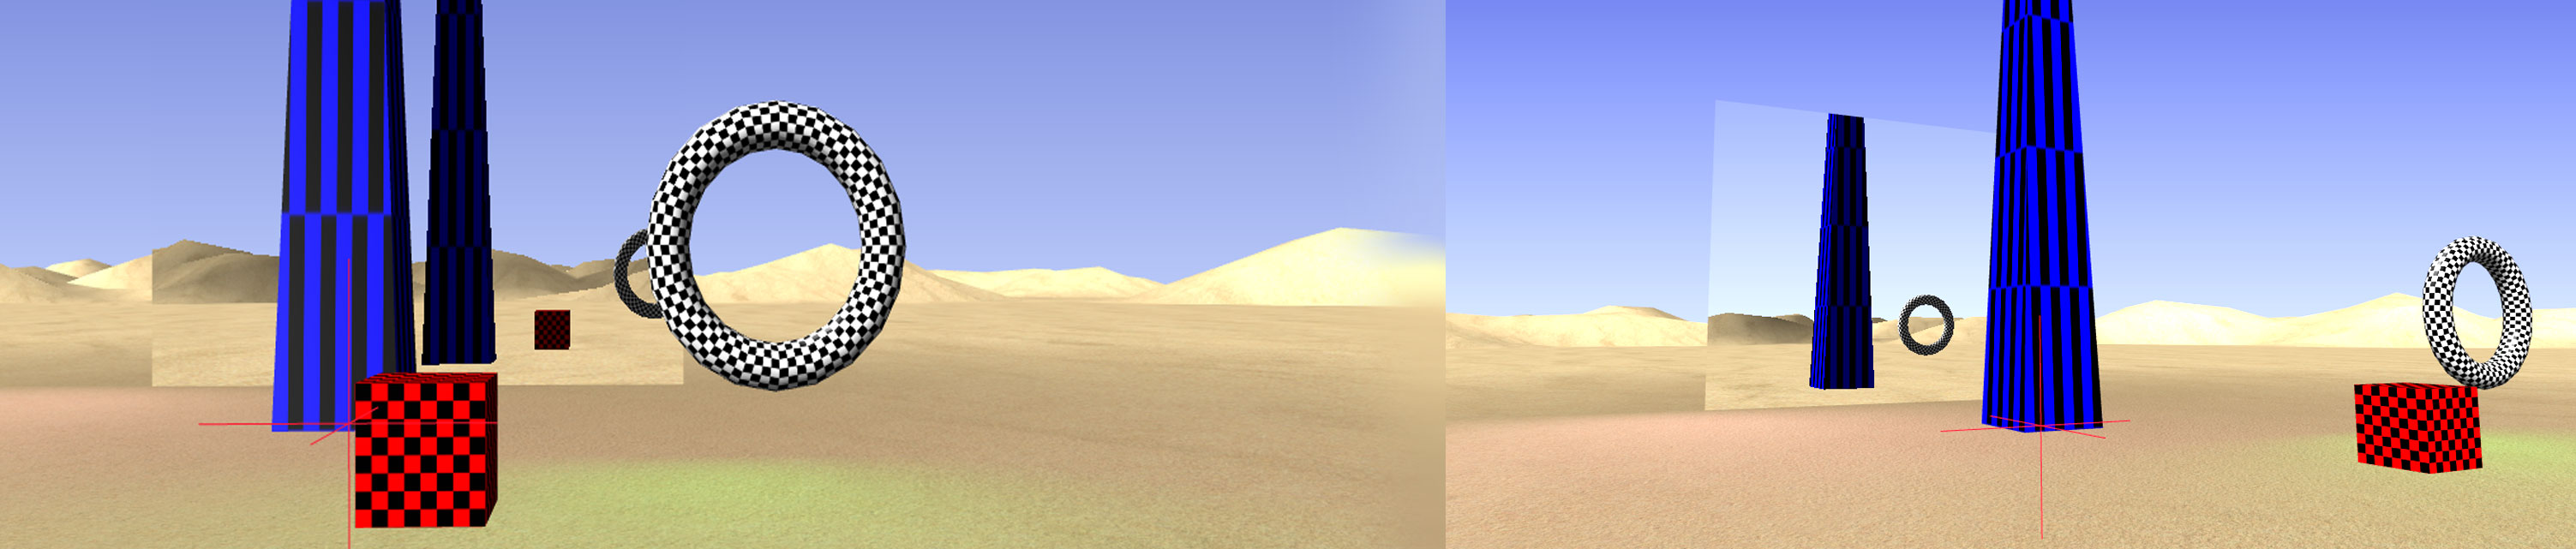
\includegraphics[height=1.5in]{images/sampleteaser}
   \caption{Project screenshot}   
 }		

\maketitle

\begin{abstract}
This project aims to develop a Real-time 3D graphics scene, with an emphasis on high aesthetic quality. The scene will use a pre-written OpenGL render framework to save development time for producing graphical effects. This project aims to also look into the cutting edge features available in the newest OpenGL standards and investigate the performance benefits of such features.
\end{abstract}

\keywordlist
%\copyrightspace

\section{Introduction}

\figuremacroW
{witness}
{Project Inspiration - The Witness}
{\protect\cite{Witness}}
{1.0}

\paragraph{Project Aims}
The setting for the project scene is a Desert. Although not a visually busy scene, a desert provides vibrant and harsh lighting, interesting landscape and plenty of opportunity to squeeze more visual fidelity out of a small amount of scene elements.
Using a multitude of texture effects, such as bump and parallax mapping, blend maps and level-of-detail, this project plans to bring life to even the most basic of objects, like sand on the ground.

\paragraph{Sky}
With the wide open vita of a desert plain, the sky takes center stage and is the most important visual cue to selling the realism of the scene. This project aims to have a fully dynamic and procedural sky system, without relying on static textures. This will allow for a time-of day system and full control of elements such as clouds and sun position.

\paragraph{Water}
The centrepiece of the scene will be a water feature of some kind, providing a contrast against the dry desert and visually interesting element in it's own right. Reflections, waves using distortion maps, refraction, and particle effects will be used to provide realistic looking water. 

\section{Background / Related Work}
\figuremacroW
{specops}
{Spec Ops: The Line}
{\protect\cite{spec}}
{1.0}
Desert scenes are not uncommon to video games, the  simplicity of the landscape was a large bonus to performance limited software.
Older games (pre DirectX 9), could get away with a simple ground mesh, a single sand texture and an interesting skybox, and this would be considered a sufficiently detailed scene for the time. See Figure: \ref{fig:GuildWars}
\\
As the graphical power of computer increased, the challenges to make a realistic desert increased dramatically, the standard of games required more than just a barren wasteland. Buildings, foliage, human characters and interesting landscape were needed and now the scene is just as complex as any other environment.
Some modern games have taken up the challenge to model sand behaviour, as a very simple fluid dynamics system to add life to a scene. Sandstorms are a popular feature as they offer the valuable benefit of obscuring level elements, these elements now do not have to be rendered, therefore increasing performance.

\figuremacroW
{GuildWars}
{Project Inspiration - Guild Wars}
{\protect\cite{GuildWars}}
{1.0}

\paragraph{Sky}
Procedural skys have been used in games for many years, the choice to use them depends on the needs of the game.  Games that have aim to have a more living environment are the primary uses for procedural skies, in other games if a static image is sufficient, then a simple texture is used.
 
\figuremacroW
{fallout3}
{Procedural Sky - Fallout 3}
{\protect\cite{fallout3}}
{1.0}

\section{Implementation}

\subsection{Sky}

\figuremacroW
{skydaigram}
{Sky Camera Calculations}
{Distance of sky is infinity}
{1.0}
Rendering the sky was achieved by rendering a single screen sized quad to the screen, set at a maximum depth to place it behind all the level elements. Calculations based on the players view matrix and the projection matrix, result in two values representing the top bop and bottom boundary of the players view. These values are a percentage between the horizontal horizon and vertical upwards view, this is used to calculate the colour of the sky at the bottom of the screen and the top. The colours are passed to the shader which interpolates between them, completing the illusion that the player is in a skydome.

\begin{lstlisting}[ caption={Sky calculations}]
  // verticle fov = 25.3125deg = 0.441786467 radians
  float verticleFov = 0.2208932335f; // vfov/2 in radians

  vec3 camview = normalize(cameraTarget - cameraposition);
  vec3 camUp = normalize(cameraUP);

  float r = atanf(verticleFov);

  vec3 topOfScrnToPlayer = normalize((r * camUp) + camview);
  vec3 bttmOfScrnToPlayer = normalize((-r * camUp) + camview);

  float topDot = dot( topOfScrnToPlayer, vec3(0, 1.0, 0));
  float bottomDot = dot( bttmOfScrnToPlayer, vec3(0, 1.0, 0));
\end{lstlisting}


\subsection{Terrain Generation}
The distant sand dunes were created by first generating a flat grid of connected polygons, this was looped through and each vertex's y value(height) was modified based on a the output of simplex noise generator. Simplex noise is an optimised version of the Perlin noise generator, both were authored by Ken Perlin, the original Perlin in 1983 and Simplex in 2001.\\
The generation happens at the start of the program and has many variables to alter the attributes of the generated terrain. As the sand dunes are far away, they are lighted with a simpler, per vertex gouraud model.

\subsection{Water}

Realistic water is made up of a multitude of components and render passes. At the simplest level, there is the reflected image from the water surface and the image of the area beneath the water surface. Each image will be combined and distorted based on the attributes of the water, the environment, and the position of the player.

\paragraph{Reflection}
At this stage in the project, only the reflection component of the water renderer has been completed, this results in the mirror effect currently in the scene. Rendering a reflection from a surface requires either using a reflection map for an approximate reflection, or re-rendering the scene from a different point, relative to the players view and position and orientation of the reflected object.
For flat surfaces, like water or a mirror, a second render pass is preferred. For complex reflective shapes, reflection maps are almost excursively used.


\figuremacroW
{reflections}
{Refection Camera position}
{\protect\cite{Riemer}}
{1.0}

\paragraph{Rendering Twice}
The position of the 'Virtual Camera' (Camera B in Figure \ref{fig:reflections}) is calulated by multiplying a reflection matrix by the view matrix of the players camera. The reflection matrix is a matrix that will mirror every position about a plane, the plane being the mirror.

\paragraph{Reflected Image}
Due to the entire coordinate system being flipped, an additional flip matrix needs to be multiplied against the Virtual camera to flip the Y elements of the polygons in the scene are facing the right direction. Alternatively, depending on the placement of the mirror, this can be avoided by simply changing which sides of faces are culled during rendering. More advanced approaches take the form of changing the virtual projection matrix to be an oblique projection with the near plane set to the mirror plane, for easier culling of geometry.

\figuremacroW
{front-Buffer}
{Rendered Scene}
{Mirror Outline overlay for clarity}
{1.0}

\figuremacroW
{ref-Buffer}
{Refection Camera View}
{UV coordinates shown, this is the area that will be rendered on the mirror quad}
{1.0}

\paragraph{Reflected Texture}
With the reflected image rendered to a texture, this image needs to be applied to the mirror geometry in the main render pass.
This process is simple in theory, the section of the image that needs to be used is the same shape as the geometry in the non reflected view.
To get this area, the positions of the geometry are transformed by the same matrices used to get the reflected view, and then this data is used as UV coordinates.

\begin{lstlisting}[ caption={Fragment Shader Reflected UV calculations}]
  vec4 reflectedPos = reflected_MVP * vec4(position.xyz, 1.0);
  vec2 transformedUV;
  transformedUV.x = reflectedPos.x/reflectedPos.w/2.0f + 0.5f;
  transformedUV.y = reflectedPos.y/reflectedPos.w/2.0f + 0.5f;
  vec4 reflectionTextureColor = texture2D (tex, transformedUV);
\end{lstlisting}

\subsection{Multiple lighting}
A simple approach to multiple lighting in a forward render solution is to send a list of appropriate lights as uniforms to a Shader.
This process must be repeated for every light in a scene and for every shader execution. Different methods are available, such as deferred rendering which separates all lighting into a completely separate render pass. The OpenGL standard mandates that all input uniforms must be a predefined size. This means that an upper limit to the amount of lights a shader can accept must be set.

\paragraph{Uniform Buffers}
A features introduced in OpenGl 3.1 is Uniform buffers. They allow data that would normally be sent to each shader at render time to be pre-stored in graphics memory. During the render, the program can inform the shader which uniform buffer to load data from. This has the primary benefit of people able to swap between different sets of static uniform data quickly, and that the data only needs to be sent once, and can be read by multiple shaders. This could be used to store all the light data in the scene efficiently.

\paragraph{Shader Storage Buffer Object}
Uniform buffers have some serious limitations, the amount of data that can be stored in them is limited and this limit varies across various hardware. This demo uses a vary small set of data for each light, so the space limitation is not an issue. However, a different type of storage introduced in OpenGL 4.3 called 'Shader Storage Buffer Objects' have no limitation on size. SSBOs also have a useful feature which is that they support variable length arrays.

\paragraph{SSBO arrays}
A program can write any length of data to an array in an SSBO, and a shader can loop through it simply by querying the size of the array using "arrayname.size()". This is not possible with any other data or storage type. This allows the program code to change the amount of lights in a scene, and update them without any interaction with shaders. This project uses this feature to demonstrate multiple lights.

\paragraph{SSBO issues}
During testing it was found that AMD graphics cards could not compile shaders that make use of the ".size()" function. The solution to this was to store the size of the array in a separate ssbo, this was read and used as the loop boundary.

\section{Future Work}

\paragraph{Sky}
The simple gradient sky will be improved with the addition of clouds and the sun. Clouds could be based form multiple layers of noise, or a particle system. Rendering the sun could be achieved with additional code to the sky fragment shader, along with some post-processing effects.

\paragraph{Water}
The existing code for the mirror will be combined with additional effects to make convincing water. To add to the effect, small ripples could propagate across the water surface, causing distortion.

\paragraph{Lighting}
More research should be done to see what can be done with SSBO's. Lights could be culled per object, and then the Index of each light that effects an object could be sent to each shader. More surface effects such as parallax mapping should also be introduced.

\bibliographystyle{acmsiggraph}
\bibliography{report}
\end{document}